\documentclass[a4paper,fleqn,usenatbib]{mnras}
%\usepackage{newtxtext,newtxmath}
\usepackage[T1]{fontenc}
\usepackage{ae,aecompl}
\usepackage{graphicx}	% Including figure files
\usepackage{amsmath}	% Advanced maths commands
\usepackage{amssymb}	% Extra maths symbols
\usepackage{hyperref}

\def\grs{{GRS\,1739-278\,}}
\def\swiftx{{\em Swift-XRT\,}}
\def\swiftb{{\em Swift-BAT\,}}
\def\xmm{{\em XMM-Newton\,}}
\def\nustar{{\em NuSTAR\,}}
\def\integral{{\em INTEGRAL\,}}
\def\maxi{{\em MAXI\,}}


\def\ferg{erg~cm$^{-2}$~s$^{-1}$}
\def\arcsec{''}
\def\degr{$^\circ$}
\def\arcmin{'}
\def\iaucirc{{IAU~Circ.}}

\title[Study of low-frequency QPO in \grs]{Study of low-frequency quasi-periodic oscillations in \grs during 2014 outburst}

%\author[I. A. Mereminskiy et al.]{
%Ilya A. Mereminskiy,$^{1}$\thanks{E-mail: i.a.mereminskiy@gmail.com}
%Andrey N. Semena,$^{1}$
%Sergey Bykov,$^{1,2}$
%Ekaterina V. Filippova$^{1}$
%\\
% List of institutions
%$^{1}$Space Research Institute, Russian Academy of Sciences, Profsoyuznaya 84/32, 117997 Moscow, Russia\\
%$^{2}$MGTU, Moscow, Russia\\
%}

\author[Authors]{
Authors$^{1}$
\\
% List of institutions
$^{1}$Space Research Institute, Russian Academy of Sciences, Profsoyuznaya 84/32, 117997 Moscow, Russia\\
%$^{2}$MGTU, Moscow, Russia\\
}


\date{Accepted XXX. Received YYY; in original form ZZZ}

\pubyear{2017}

\begin{document}
\label{firstpage}
\pagerange{\pageref{firstpage}--\pageref{lastpage}}
\maketitle

\begin{abstract}
\end{abstract}
We detected low-frequency quasi-periodic oscillations (QPOs) at 0.3..2 Hz in \nustar and \swiftx observations of black hole candidate \grs during its 2014 outburst.

\begin{keywords}
X-rays: individual (\grs)  -- accretion, accretion disks	
\end{keywords}


\section{Introduction}
\label{sec:intro} 
The study of rapid X-ray variability is important, indeed.

\section{GRS 1739-278}

\grs is a typical X-ray nova, discovered during outburst in 1996  \citep{paul96} by SIGMA \citep{paul91} telescope onboard GRANAT space observatory.
Using {\it ROSAT} observation \cite{greiner96} inferred distance of 6--8.5~kpc, indicating that source may belong to Galactic bulge. 	

%\grs was discovered in 1996 by SIGMA telescope onboard GRANAT space observatory  \citep{paul96}.  
%Later GRANAT continued observations of this source \citep{vargas97} along with other X-ray telescopes: ROSAT \citep{greiner96}, RXTE and TTM/Kvant \citep{borozdin98}. The optical counterpart was found in observations carried out by ESO telescopes \citep{marti97}. . During the outburst \grs demonstrated typical behavior of the black hole candidate \citep[BHC, see e.g.][]{grebenev93, grebenev97, tanaka96, remillard06, belloni10}. The lightcurve could be described with a FRED-like (fast rise, exponential decay) shape, at the beginning of the outburst the source was in a typical low/hard state, with spectrum dominated by a power-law component with exponential cutoff at high ($\ge$100 keV) energies followed by a high/soft state with a strong blackbody component \citep{borozdin98}. Observations at VLA \citep{hjellming96} revealed presence of variable radio emission, which could be caused by jets.  \cite{borozdin00} found QPO at 5 Hz in RXTE observations conducted while the source was in the very high/soft state.

%The onset of 2014 outburst was detected by \swiftb \citep{krimm14_atel} along with \integral \citep{filippova14}. 

%At the beginning of the September, 2016 there was another, third, outburst, that 

\begin{figure*}
\centerline{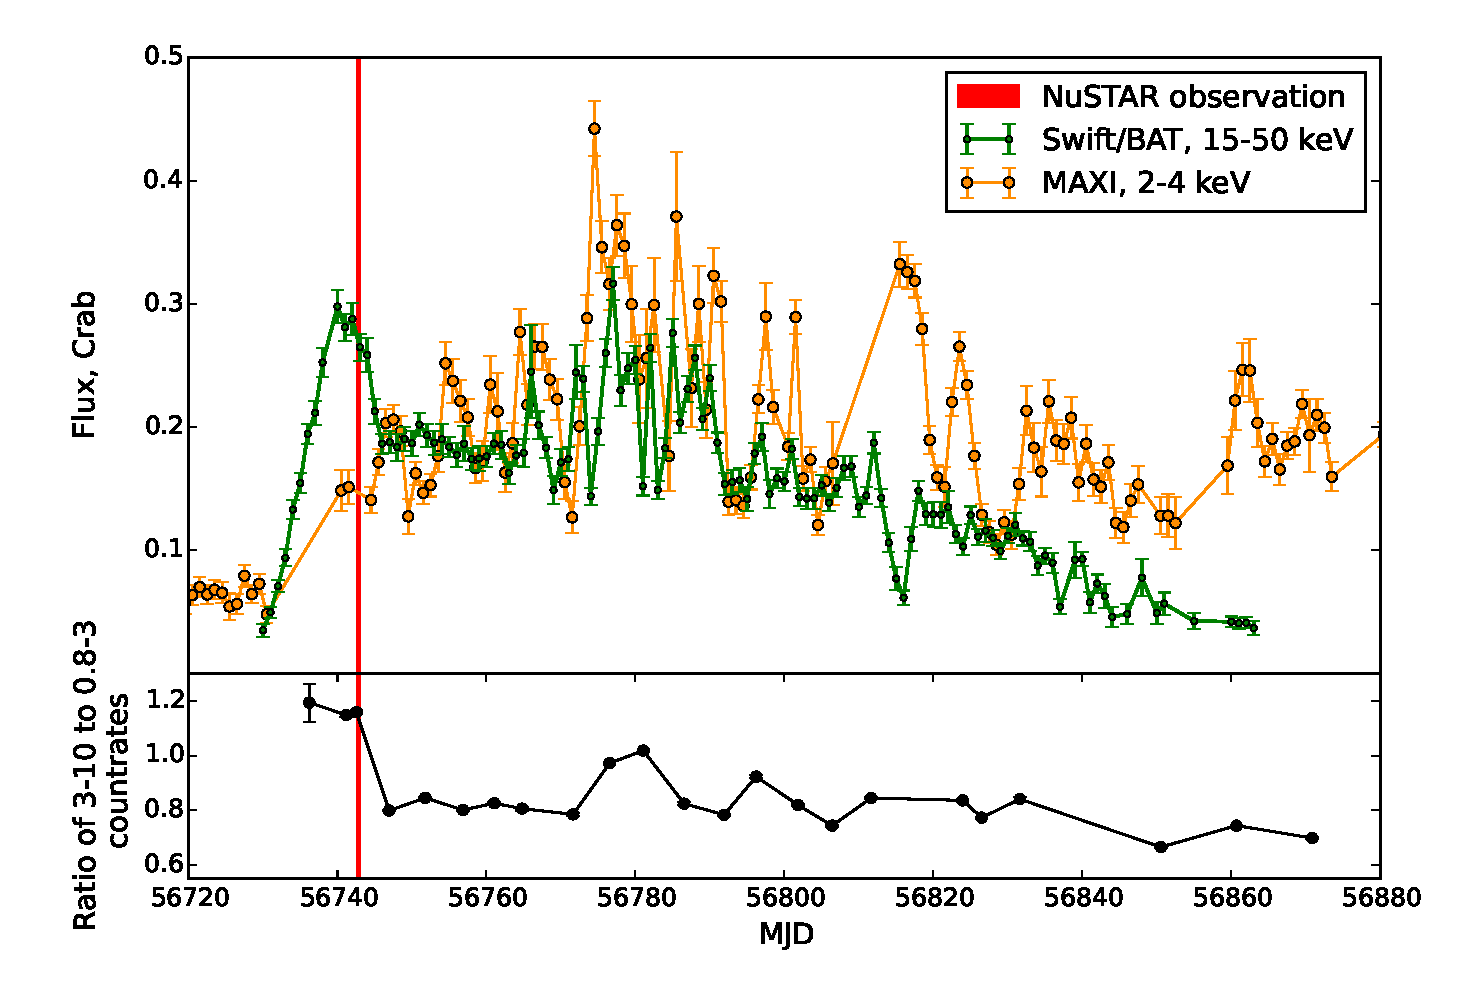
\includegraphics[scale=0.5]{batlc_v06.eps}}
\caption{{\it Upper:} green points denote \swiftb\, lightcurve of second outburst in 15--50 keV range, orange circles correspond to \maxi\, fluxes in 2--4 keV. Red line show time of \nustar\, observation. {\it Lower:} evolution of \swiftx\, spectral hardness during the outburst.} 
\label{fig:batlc}
\end{figure*} 

\section{Observations and data reduction}
\label{sec:datared} 
In order to characterize the overall outburst profile we used data of \swiftb\, {\it transient monitor} \citep{krimm13bat} in hard X-rays (15--50 keV) as well as data from \maxi\, \citep{matsuoka13maxi} (2--4 keV).

We used public observations of \swiftx\, (target ID: 33203) performed regular over the peak and decline of the outburst.  Since the source was bright, all \swiftx\, observations were performed in windowed mode, allowing study of timing properties of the source. We performed standard analysis with {\texttt{xrtpipeline}} and barycentered data prior to lightcurve extraction. 
Long-term lightcurves were obtained from UK Swift Science Data Centre at the University of Leicester \citep{evans09}.

We also used \nustar\, observation (ObsID: 80002018002) performed at March 26, 2014 (MJD 56742).  {\texttt{Nuproducts}} pipeline were utilized to extract photons  from two-arcminute circular region, centered on source and to produce lightcurves and spectra.

\section{Analysis}
\subsection{Outburst}
First detection of the source by \swiftb\, \citep{krimm14_atel} occurred at March 9, 2014 (MJD 56725, we will refer to this date as $\tau_{0}$), onset of outburst was the confirmed by \integral\, \citep{filippova14}. Outburst profile in hard X-rays (15--50~keV) featured fast rise with tenfold intensity increase over ten days, nearly flat-top peak ($\tau_{0}$+10..+15) followed by abrupt flux decrease by 30\% over two days. After this, source demonstrated gradual decline interrupted by flaring activity at $\tau_{0}$+30..+65. Another interesting feature is dip, observed in \swiftb\, lightcurve at $\tau_{0} \approx 86$. After the cease of the outburst source remained active with flux about 5--15 mCrab. 

Adding softer data from \maxi\, to the \swiftb\, hard X-ray lightcurve gives us another insight on evolution of the outburst as shown in Fig.\,\ref{fig:batlc} - comparing fluxes in soft and hard bands (for 2--4 keV band we took a 1.67 counts s$^{-1}$ as a reference value for Crab, corresponding value for 15--50 keV band is 0.22 cts cm$^{-2}$ s$^{-1}$) one can see that soft component obviously lags hard emission in the beginning of the outburst but then start to grow and ends up dominating during the flaring period as well as hard dip(s). Lower subplot of Fig.\,\ref{fig:batlc} shows evolution of hardness ratio (3--10~keV/0.8--3~keV) measured by \swiftx. Right after peak of hard X-rays one can see decline of hardness, also indicating appearance of thermal component.

This type of behavior is typical for black hole candidates \citep[BHC, see e.g.][]{grebenev97, tanaka96, remillard06, belloni10} - outburst starts from low-hard state (LHS) moves through hard intermediate state (HIMS), then proceeds to the high-soft (HSS) (or even very-high-soft state, as were seen in 1996 outburst \citep{borozdin00}) and then returns back to LHS and, eventually, to quiescence.

Fortunately, the \nustar\, \citep{harrison13_nust} observation triggered by \cite{miller15_nust} were carried right at the transition between hard and soft states, thus giving us unique possibility to study processes that happens during HIMS. 

\subsection{NuSTAR observation}
\label{sec:nust} 

\nustar\, observed \grs (ObsID: 80002018002) for nearly 30 ks of dead-time corrected exposure right after hard X-ray peak (see Fig.~\ref{fig:batlc}). Earlier, \cite{miller15_nust} shown that the average spectrum of this observation is well described by reflection models such as {\it relxill} \citep{garcia14, dauser14,dauser16} with accretion disk that reaches remarkably close to the black hole innermost stable circular orbit (ISCO), with upper estimate being $r_{in} = 5^{+3}_{-4}\, G M/c^{2}$ \citep{miller15_nust}. Interestingly, no additional thermal component was needed in order to obtain a good fit, probably because of \nustar\, energy band, starting at 3~keV. 

Given the 96.9 minute orbital period of \nustar, observation is divided in 13 intervals separated by Earth occultations, as shown in Fig.\,\ref{fig:nust_lc}. We denoted this intervals with roman numerals, from {\bf I} to {\bf XIII}. From the lightcurve of observation it is clear, that source flux is increasing throughout observation from $\approx$145 counts per second up to $\approx$170 counts per second. 
The spectrum also alter, with hardness (defined as ratio of countrates  $R_{3-10\,keV}/R_{10-78\,keV}$) monotonically growing from 2.5 to 3.5. 
Since it is obvious that the source spectrum is somehow changing during the observation it is interesting to check if Fe-line profile stays the same during observation or changes. 
We split observation into three major pieces, with first made by intervals {\bf I-IV}, second by {\bf V-IX} and third by {\bf X-XIII} and extracted 3--78 keV spectra. 
We chose to group them in order to have at least 100 counts per bin. 
Then we fitted them using \texttt{XSPEC} package \citep{arnaud96} (excluding data below 4 keV and between 5--10 keV) with simple \texttt{phabs*cutoffpl} model, using $N_{H} = 2.15\times10^{22}$ cm$^{-2}$ as was found by joint \xmm/\nustar\, observation during low luminosity state \citep{fuerst16}. Element abundances were taken from \cite{wilms00} and cross-sections from \cite{verner96}. Now, plotting the ratio of this fit to initial spectra (see Fig.~\ref{fig:ratios}) one can see that both strong features - i.e. Fe-line complex at 5--9 keV and Compton hump around 30 keV are seemingly stable. 

\begin{figure*}
\centerline{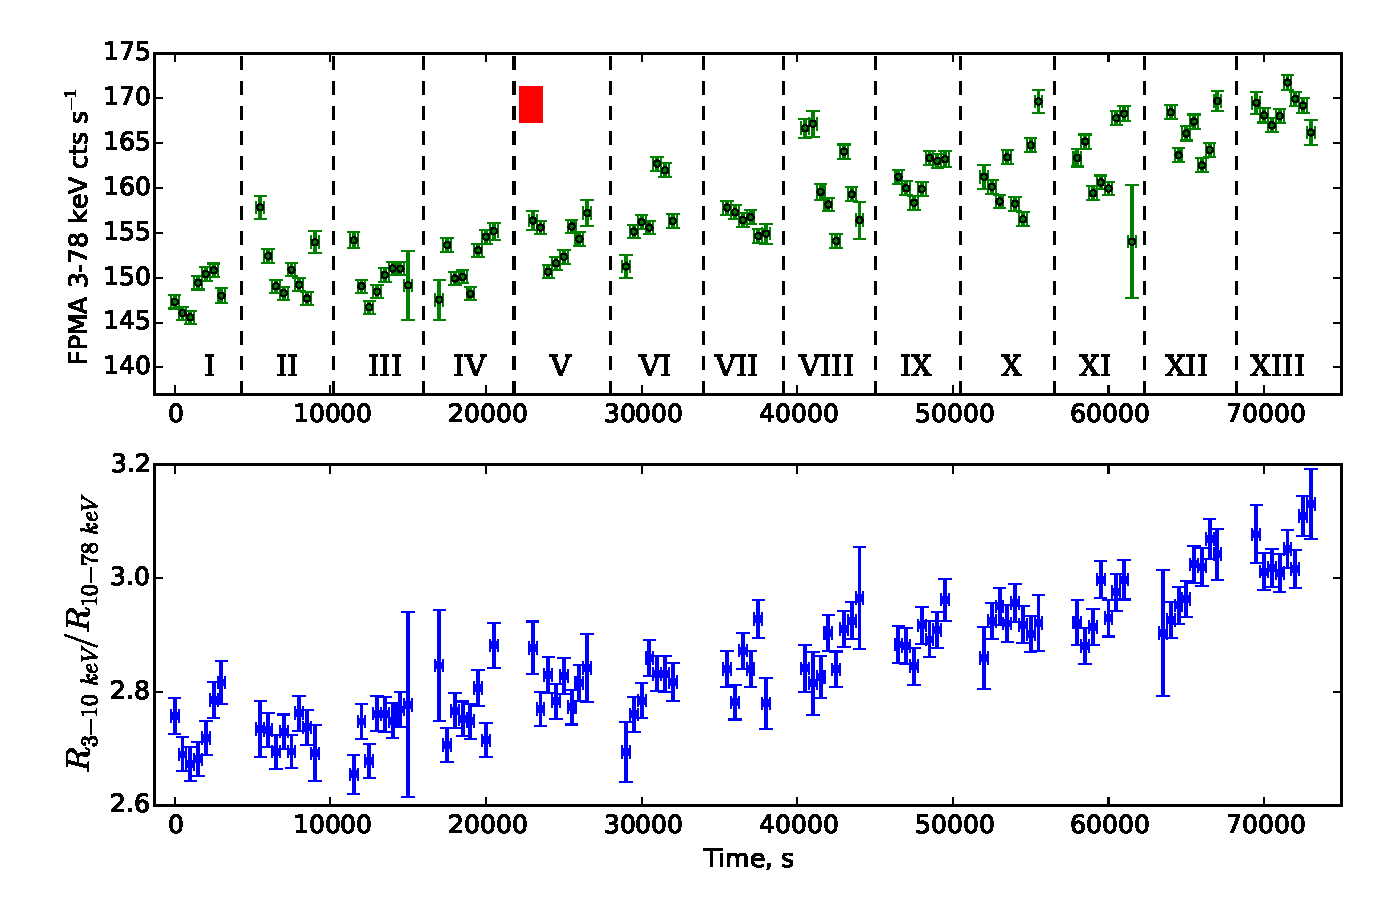
\includegraphics[scale=0.7]{nuAlc_color_v04.eps}}
\caption{Upper panel: countrate of \nustar\,FPMA in 3--78 keV band. We enumerated intervals of uninterrupted observations with roman numerals. Red square shows time of simultaneous \swiftx observation (ObsId: 00033203003, second part). Bottom panel: evolution of hardness during observation} 
\label{fig:nust_lc}
\end{figure*} 
 \begin{figure}
\centerline{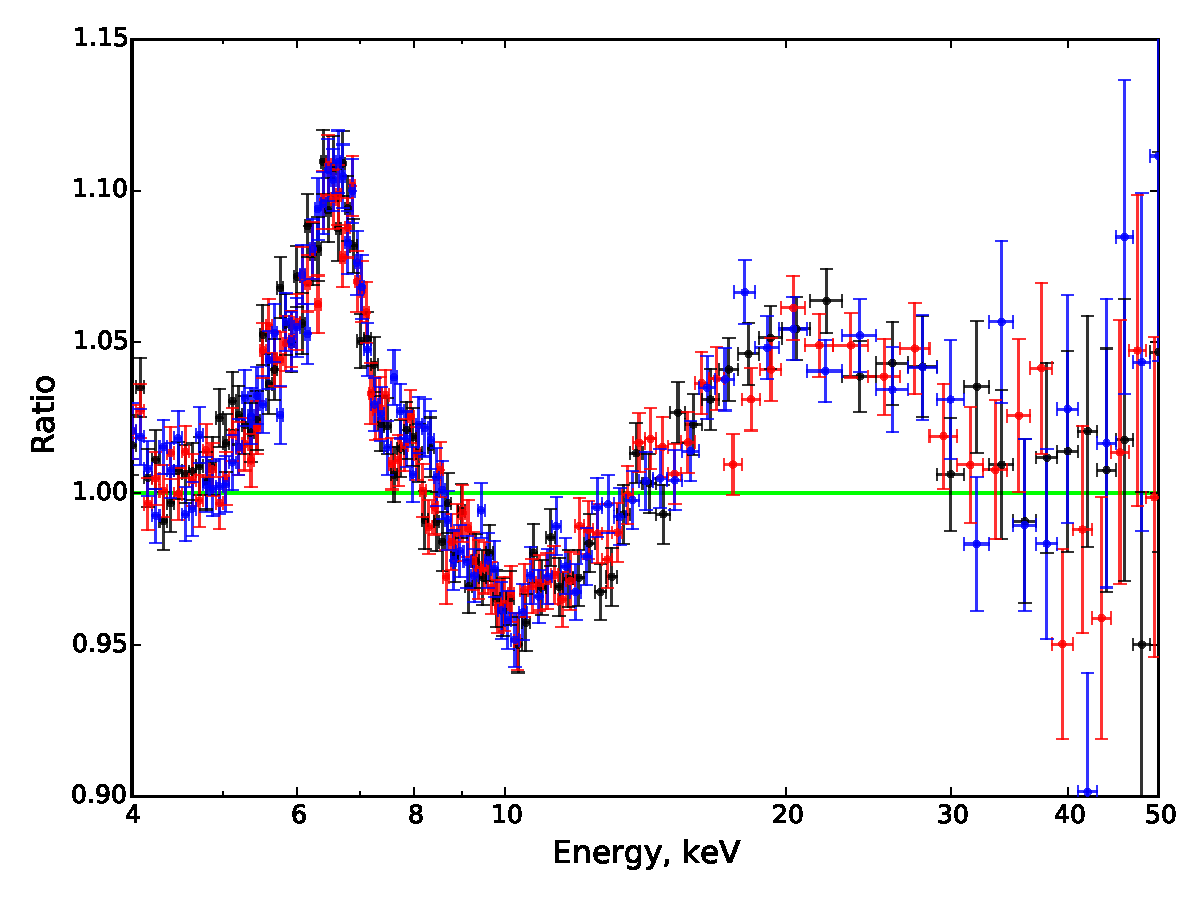
\includegraphics[width=\linewidth]{ratios_v01.pdf}}
\caption{Ratio of \nustar\, spectra to \texttt{phabs*cutoffpl} model. In black - data from intervals I-IV, in red from V-IX and in blue from X-XIII.} 
\label{fig:ratios}
\end{figure}  

To get better view on evolution of continuum emission we fitted all individual interval spectra with \texttt{xillver} model \citep{garcia13}. This model describes reflection of incident radiation from ionized slab of matter. The spectrum of incident radiation are assumed to be power-law with exponential cutoff. Spectra from two \nustar\, modules from each interval were fitted simultaneously with \texttt{phabs*const*xillver} model. We choose to fix interstellar absorption at $N_{H} = 2.15\times10^{22}$ cm$^{-2}$. Relative iron abundance were fixed at
 $A_{Fe} = 1$, ionization parameter at $\xi=3.2$ and inclination at 35 degrees. This parameters are in agreement with measured by \cite{miller15_nust} with different spectral models. Although in  \texttt{xillver} there is no relativistic broadening of Fe-line no significant residuals in 5--8 keV region are seen, mainly because of limited statistics in per interval spectra. Before fitting, spectra were grouped in order to have at least 100 counts per bin, channels above 60 keV were ignored. Resulting fits are of satisfactory quality with mean $\chi^{2}_{red.} \approx 1.05$. 
 
Examination of best-fit parameters shown in Fig.\ref{fig:intspe} confirms that spectrum softens during observation and cut-off energy decreases. Flux is steadily increasing and at the end of observation unabsorbed luminosity in 3--60 keV band reach  $7\times10^{37}$ erg s$^{-1}$ assuming 8 kpc distance.

\begin{figure}
\centerline{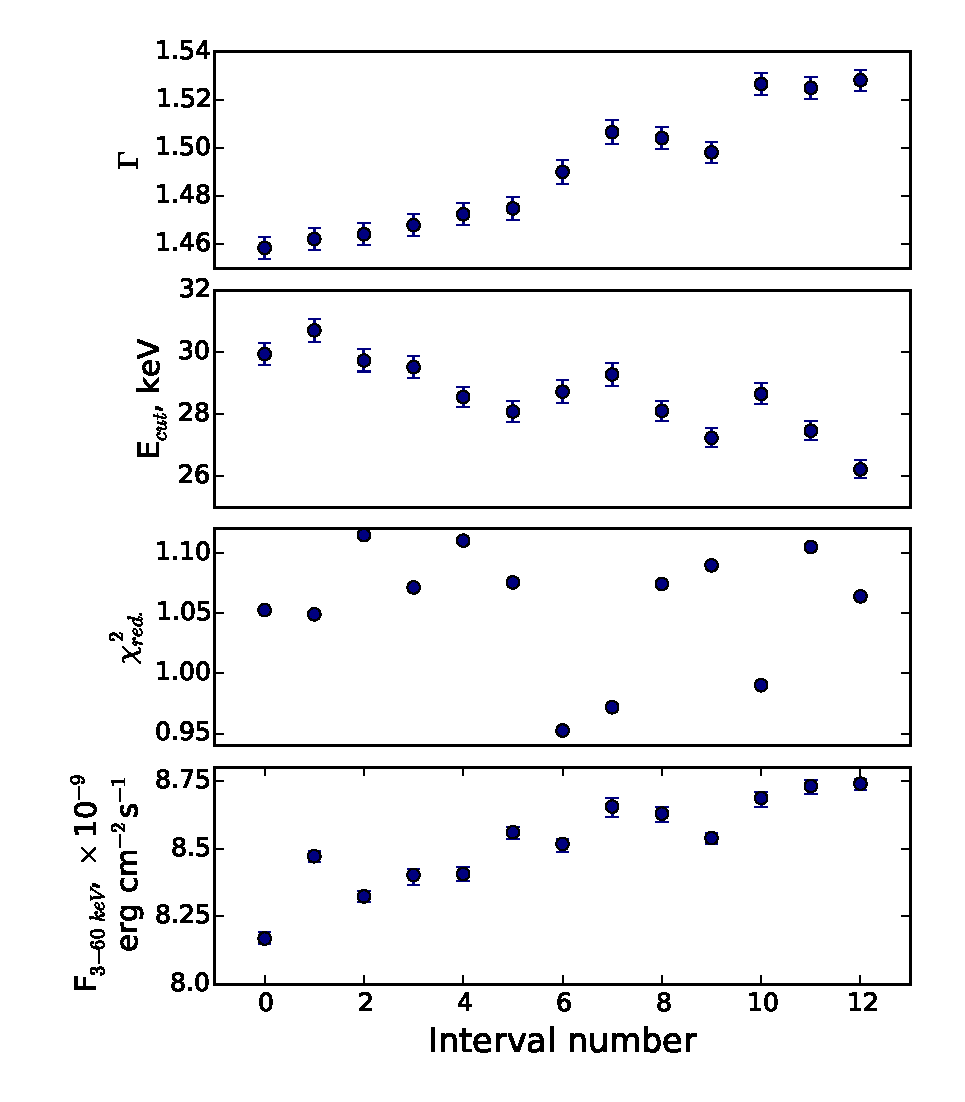
\includegraphics[width=\linewidth]{intspe_v01.eps}}
\caption{Parameters of continuum emission in intervals. } 
\label{fig:intspe}
\end{figure}  
            
There is a 1 ks part of \swiftx\, snapshot (ObsId: 00033203003) that coincides with \nustar\, observation.  Extending energy range to 0.8 to 78 keV allow one to search for thermal emission associated with cold inner disk with $kT \sim 0.1...0.4 keV$ (such as were found in other BHCs, see \cite[][ e.t.c]{miller06b,miller06a,parker15}).
We used latest available version of {\it relxill} package (v1.0.2). 
Element abundances were taken from \cite{wilms00} and cross-sections from \cite{verner96}.


%\begin{figure*}
%\centerline{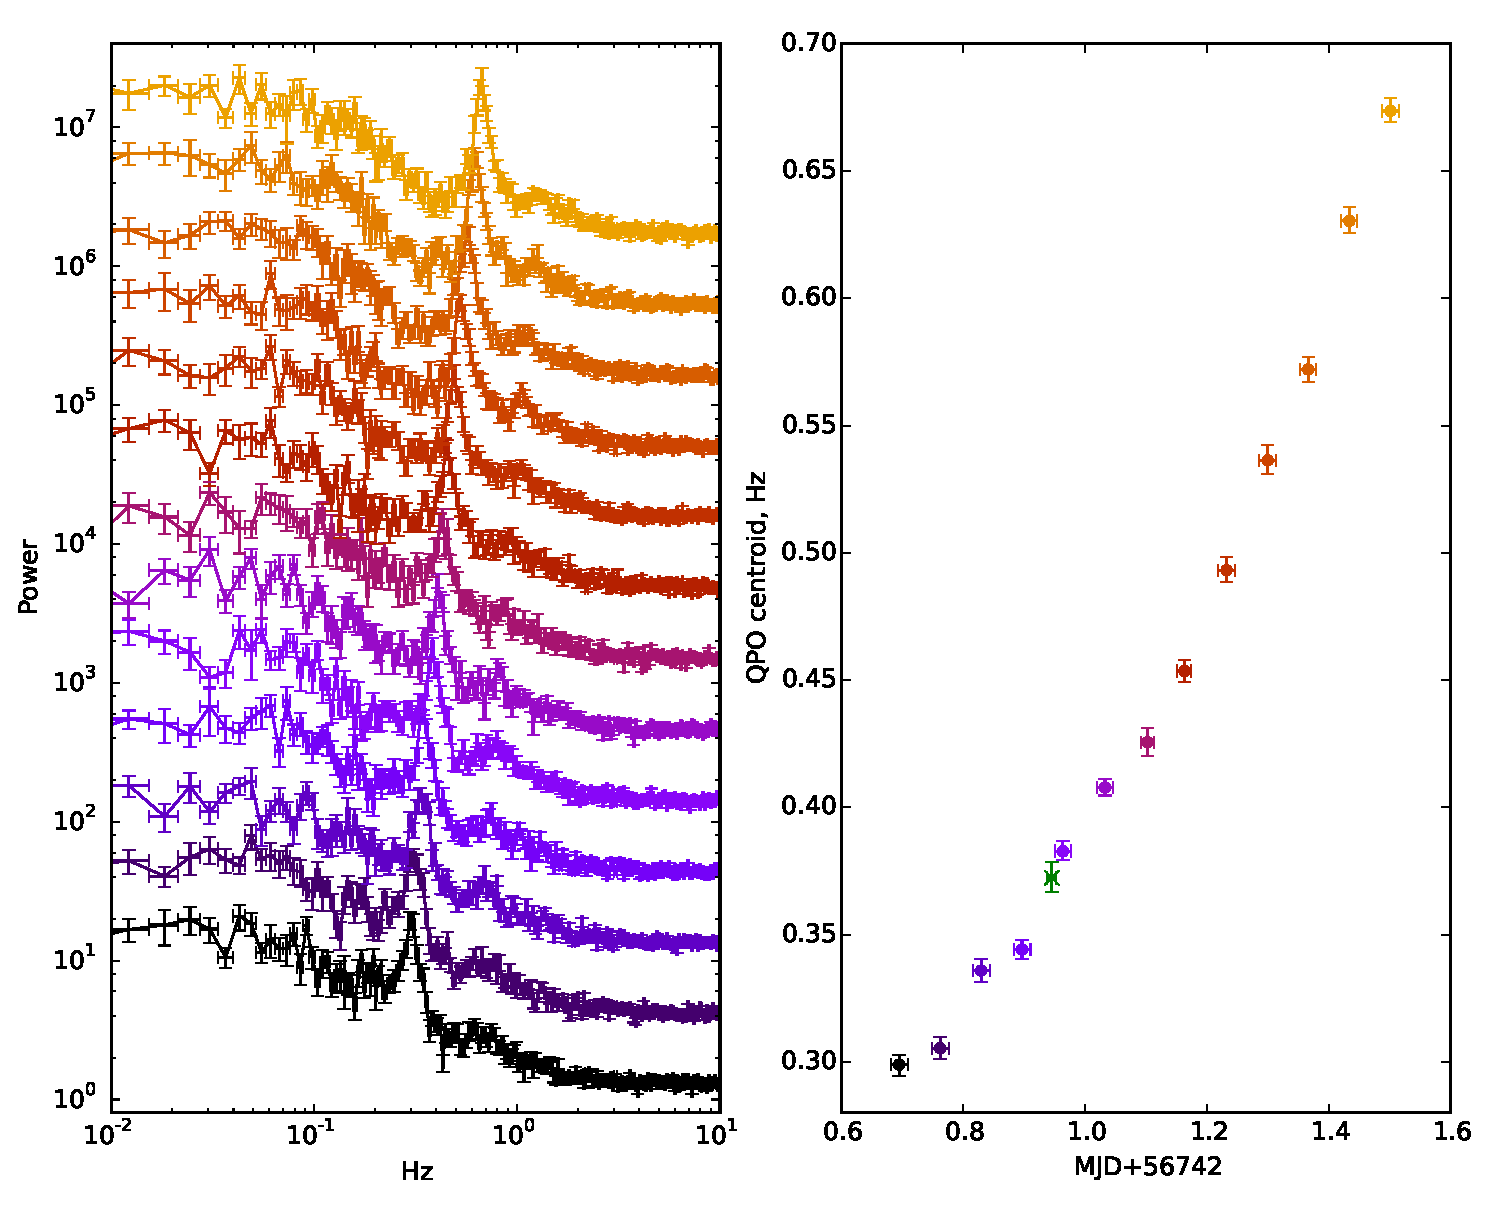
\includegraphics[scale=0.7]{QPOdrift_v02.eps}}
%\caption{Change of the QPO frequency with time. On the left panel we show how power-density spectra change with time - for clarity each spectrum is multiplied by a factor of 3.25. On the right panel we show how the QPO frequency changes during observation. Green cross show QPO frequency derived from \swiftx\, observation.} 
%\label{fig:qpodrift}
%\end{figure*}  


\section{Timing analysis} 

    Along with the spectral analysis of X-ray transients, timing analysis give a vast of information about the geometry and current state of the accretion flows in such systems. 
For example, broad band timing variability properties are used in determination of the systems state \cite{2005Ap&SS.300..107H}.

    Variability properties of different types of X-ray binary systems are usually described in terms of the luminosity power spectrum, which is a common technique on determination of amount of power in the particular frequency range.
    Luminosity variability power spectrum of the transient system typically can be described with a set of broad and thin Lorentzian functions representing correspondingly broad band stochastic noise and QPOs \citep[see, e.g.][]{1972ApJ...174L..35T, 1990A&A...227L..33B}.
    The overall variability and the shape of the power spectrum changes dramatically with the spectral states of the transients and, in some cases, manifest state transitions even if they are not evident from the energy spectrum.

    Some aspects of the evolution of the X-ray binaries system power spectrum with their state can be explained in the frame of the two-temperature accretion flow model, where it consists of the geometrically thin cold disk and geometrically thick hot flow (corona), particularly it is widely accepted that the high amplitude variability is associated with the geometrically thick flow, while the geometrically thin disk is generally stable \citep{2001MNRAS.321..759C}. 
It should be noted that this model of the variability generation are directly connected with the models, explaining energy spectra of black hole binaries \citep[see, e.g.,][]{1975ApJ...199L.153E, 1976ApJ...204..187S, 1995ApJ...452..710N}, \citet{2001MNRAS.321..759C} has shown with the frequency resolved spectroscopy that variable part of the emission has a hard spectrum, which is thought to be produced in the corona, while stable part of the emission has a spectrum which is consistent with the cold classical $\alpha$-disc spectrum \citep{ss73}.

    It is generally accepted that the broadband noise observed in the power spectrum of binary systems is produced due to the stochastic variations of the angular momentum transport efficiency \citep{1997MNRAS.292..679L}. 
    In this propagating fluctuation model broad band noise is a product of noisy signals from different radii of the accretion flow, each with its own characteristic time-scale \citep[see, e.g.][]{2006MNRAS.367..801A, 2013MNRAS.434.1476I}.
    It follows, that the shape of the broad band noise is determined with the physical and geometrical properties of the accretion flow, e.g. in particular in these works it was suggested that the broad noise dumping frequency is connected to the accretion flow inner edge.

    Another feature, frequently observed in the X-ray binaries power spectra is different types of low and high frequency QPOs manifesting itself as an excessive power in the thing frequency bands. 
    There is at least five types of these QPOs were observed on the frequencies above 0.1~Hz in the stellar mass binary systems \citep[for classification see][]{2005Ap&SS.300..107H}.

Several models were proposed to explain high and low frequency QPO features in power spectra \citep[][]{1997ApJ...489..865E, 1998ApJ...506..281B, 1998ApJ...492L..59S, 1999A&A...349.1003T, 1999ApJ...518L..95T, 2001A&A...374L..19A, 2009MNRAS.397L.101I, 2011MNRAS.415.2323I}. 
Changes, observed with the evolution of the spectral states between different types QPOs and broad band noise, e.g. correlation between QPOs centroid frequencies and broad noise dumping frequency \citep{1999ApJ...514..939W, 2014MNRAS.437.2554M} speak in favor of the origin of the QPOs in the inner edge of the accretion flow.

While these models, describing broad band noise and QPOs in the variability power spectrum, usually do not confront observed energy spectra, it was found that some additional demands on time properties must be met.
\citet{1997ApJ...474L..43V} used coherence spectrum in order to additionally constrain time properties of the accretion flow. 
They found a time lag between hard and soft emission of the soft and hard emission, which have a complex behaviour with the frequency, which they used to constrain geometrical size of the accretion flow \citep{1999ApJ...517..355N}. 
Observed time lags also were used to discriminate some spectral models \citep[see, e.g.,][]{2001MNRAS.327..799K}.

In the following section we presenting analysis of the timing properties and their evolution of \grs\ during the 2014 outburst.
%Most of that models were architect in order to explain energy spectra (or particular feature in it) and the power spectra. 
%However, as will be discussed in the following chapter, additional analysis, describing time properties in different energy bands, can be applied to rule out some of that models.

\begin{table*}
\noindent
\centering
\caption{Evolution of the Fourier and energy spectrum properties through the {\it NuSTAR} observation in the 3--5~keV energy band.}
\label{tab:timing}
\centering
\begin{tabular}{|c|c|c|c|c|c|c|c|c|c|c|}
\hline\hline
Data set & Tstars, s & duration, s & f$_{\rm br}$, Hz & f$_{\rm qpo}$, Hz & Q$_{\rm m}$ & A$_{\rm m}$, (rms/mean) \% & A$_{\rm o}$, (rms/mean) \%i & rms, \% & $\Gamma$ & E$_{\rm cut}$, keV \\
\hline
I & 2014-03-26 16:19:55.687 & 3386 & $(9.0\pm2.5)\times10^{-2}$ & $0.30\pm0.01$ & $7.2_{-1.8}^{+2.5}\times10^{-2}$ & $7.4_{-1.2}^{+1.1}$ & $3.9_{-1.3}^{+1.1}$ & $27\pm3$ & $(145.9\pm0.5)\times10^{-2}$ & $29.9\pm0.4$ & \\
II & 2014-03-26 17:56:50.257 & 3388 & $8.8_{-2.3}^{+2.6}\times10^{-2}$ & $0.31\pm0.01$ & $8.5_{-2.2}^{+2.6}\times10^{-2}$ & $7.6\pm1.2$ & $3.3_{-1.2}^{+1.1}$ & $24_{-2}^{+3}$ & $(146.2\pm0.5)\times10^{-2}$ & $30.7\pm0.4$ & \\
III & 2014-03-26 19:33:44.826 & 3392 & $9.1_{-2.2}^{+3.2}\times10^{-2}$ & $0.34\pm0.01$ & $8.7_{-2.2}^{+3.3}\times10^{-2}$ & $7.2\pm1.2$ & $3.9_{-1.2}^{+1.0}$ & $26\pm3$ & $(146.4\pm0.5)\times10^{-2}$ & $29.7\pm0.4$ & \\
IV & 2014-03-26 21:10:39.396 & 3389 & $8.3_{-2.1}^{+2.5}\times10^{-2}$ & $0.35\pm0.01$ & $8.6_{-1.9}^{+2.4}\times10^{-2}$ & $7.3_{-1.2}^{+1.1}$ & $4.2_{-1.2}^{+1.1}$ & $27_{-3}^{+4}$ & $(146.8\pm0.5)\times10^{-2}$ & $29.5_{-0.3}^{+0.4}$ & \\
V & 2014-03-26 22:47:33.966 & 3389 & $7.2_{-1.9}^{+2.0}\times10^{-2}$ & $0.39\pm0.01$ & $8.6_{-2.1}^{+2.7}\times10^{-2}$ & $7.1_{-1.1}^{+1.0}$ & $4.4_{-1.3}^{+1.2}$ & $27_{-3}^{+4}$ & $(147.3\pm0.5)\times10^{-2}$ & $28.6\pm0.3$ & \\
VI & 2014-03-27 00:28:41.566 & 3136 & $7.2_{-2.0}^{+2.1}\times10^{-2}$ & $0.41\pm0.01$ & $7.1_{-1.8}^{+2.0}\times10^{-2}$ & $7.0\pm1.1$ & $4.8_{-1.2}^{+1.1}$ & $27_{-3}^{+4}$ & $(147.5\pm0.5)\times10^{-2}$ & $28.1\pm0.3$ & \\
VII & 2014-03-27 02:11:38.186 & 2771 & $8.4_{-2.2}^{+2.5}\times10^{-2}$ & $0.42\pm0.02$ & $0.13_{-0.03}^{+0.04}$ & $7.3_{-1.3}^{+1.2}$ & $4.1_{-1.2}^{+1.4}$ & $25_{-3}^{+4}$ & $1.5\pm0.0$ & $28.7\pm0.4$ & \\
VIII & 2014-03-27 03:38:17.676 & 3387 & $6.0_{-1.7}^{+1.8}\times10^{-2}$ & $0.46\pm0.01$ & $7.2_{-1.9}^{+2.5}\times10^{-2}$ & $6.6_{-1.0}^{+1.1}$ & $3.8_{-1.3}^{+1.1}$ & $30_{-5}^{+6}$ & $(150.7\pm0.5)\times10^{-2}$ & $29.3\pm0.4$ & \\
IX & 2014-03-27 05:15:12.246 & 3392 & $0.13\pm0.03$ & $0.49\pm0.02$ & $0.15_{-0.03}^{+0.04}$ & $9.8_{-1.1}^{+0.9}$ & $6.6_{-1.2}^{+1.0}$ & $21\pm1$ & $(150.4\pm0.5)\times10^{-2}$ & $28.1\pm0.3$ & \\
X & 2014-03-27 06:52:06.816 & 3390 & $7.9_{-2.5}^{+2.4}\times10^{-2}$ & $0.54\pm0.01$ & $7.8_{-1.8}^{+2.1}\times10^{-2}$ & $7.9_{-1.0}^{+1.1}$ & $5.3_{-1.0}^{+1.2}$ & $26_{-3}^{+5}$ & $(149.8\pm0.5)\times10^{-2}$ & $27.2\pm0.3$ & \\
XI & 2014-03-27 08:29:02.385 & 3382 & $6.3_{-1.9}^{+2.3}\times10^{-2}$ & $0.57\pm0.01$ & $7.8_{-1.7}^{+2.0}\times10^{-2}$ & $8.3\pm1.0$ & $4.1_{-1.4}^{+1.1}$ & $26_{-3}^{+5}$ & $152.7_{-0.5}^{+0.4}\times10^{-2}$ & $28.7\pm0.3$ & \\
XII & 2014-03-27 10:05:56.965 & 3386 & $7.1_{-2.2}^{+2.4}\times10^{-2}$ & $0.63\pm0.01$ & $8.8_{-1.7}^{+2.7}\times10^{-2}$ & $8.9_{-1.1}^{+1.0}$ & $5.1_{-1.3}^{+1.2}$ & $26_{-3}^{+6}$ & $(152.5\pm0.4)\times10^{-2}$ & $27.5\pm0.3$ & \\
XIII & 2014-03-27 11:42:51.535 & 3391 & $6.8_{-2.1}^{+2.2}\times10^{-2}$ & $0.67\pm0.01$ & $6.5_{-1.4}^{+2.0}\times10^{-2}$ & $8.8_{-0.9}^{+1.0}$ & $4.4_{-1.2}^{+1.1}$ & $27_{-4}^{+6}$ & $(152.8\pm0.4)\times10^{-2}$ & $26.2\pm0.3$ & \\

\hline
\end{tabular}
\end{table}
\subsection{Power spectrum}
    {\it NuSTAR} observation of the \grs\ 2014 outburst are split on 13 continuous parts separated with $\sim0.7$~hr intervals when the source was occulted by Earth. 
    The continuous observations have duration from $\sim2440$ to $\sim3390$~sec see Table~\ref{}.
    Since {\it NuSTAR} detectors operate in the photons counting mode, data can be reduced to the light-curve with time resolution up to 2$\mu$s.
    For our analysis we extracted light-curves with 0.01~s temporal resolution, therefore we obtained power spectra in the $sim3\times10^{-3}$--$50$~Hz range.
    This is a frequency range which usually contains low frequency quasi periodic oscillations QPOs and broad band noise component \citep{1999ApJ...514..939W}.
    We didn't try to found high frequency QPOs, since the typical HF QPO (centroid frequency 100-400~Hz, amplitude $\approx10$\% and quality $Q\approx0.1$--$0.5$) is indiscernible over the Poisson noise with the obtained count-rate.

    The power spectrum of each of the separate observations has a form of a white noise plateau ($P(f)\propto const$) on the low frequencies, transforming on the frequency $\approx0.1$~Hz in to the power law with the slope $\rho\approx-1.6$--$-2.0$. 
    Also a prominent QPO on the frequencies 0.3--0.7~Hz and its second overtone is presented.
    Poisson noise dominates intrinsic source variability on the frequencies over $\approx2$~Hz, preventing analysis of any high-frequency features. %, nevertheless we inspected power spectrum in the range from 100 to 500~Hz and didn't find any signs of high frequency QPOs.
    There is also signs that the Power spectrum on the frequencies below $\approx0.003$~Hz has a form of growing power law $P(f)\proptof^{\alpha}$, $\alpha > 0$.

    From the shape of the energy and Fourier spectrum we concluded that the system is in the hard intermediate state and observed low frequency QPO (LF QPO) is of type C. 

    In order to assess properties of the variability power spectra we approximate each obtained power spectra with the following analytical function:
\begin{equation}
        \begin{split}
        P(f) = n (1 + (f/f_{\rm lb})^4)^{\alpha} + \\
        \frac{s_1}{(f - f_{qpo})^2 + (f_{\rm qpo} Q_{\rm m})^2} +\\
        \frac{s_2}{(f - 2f_{qpo})^2 + (2f_{\rm qpo} Q_{\rm m})^2} + \\
        + poiss
\end{split}
        \label{eq:complex_fit}
\end{equation}


In this function first component represents plateau with the break which can be sharp or smooth, second two components describe QPO main harmonics and its overtone, fourth component represents any additional high frequency power, it can describes either detector dead time effects or broad featureless component connected to the QPO power spreading to the high frequencies, last component represents constant Poisson noise.

Due to the complex dead-time behaviour over the energy, it's impact on to the power spectrum can not be well described. 
\citet{2015ApJ...800..109B} proposed to use real part of the cross-product between two independent {\it NuSTAR} detectors for the power spectrum assessment ($P(f)\approx real(F(f)_{\rm fpma}^{*}F(f)_{\rm fpmb}$, where $F(f)_{\rm fpma}$ and $F(f)_{\rm fpmb}$ - are measured Fourier signal on corresponding frequency $f$ and $^{*}$ - complex conjugation operation) in order to read out of Poisson noise and dead time effects.
This method is based on the following assumption: since photons arrival times are independent for the two detectors, phases of the Fourier function of two light-curves are also random and independent.
It follows that this cross-product is a complex value with random uniformly distributed phase and the mean of it's real part is zero.
Following \cite{2015ApJ...800..109B} we calling obtained function cross-spectrum or cospectrum. 

While cross-spectrum technique works perfectly for the power spectrum assessment, we still using classical Fourier power spectrum for the analysis in this work due to the following reason.
Each value of the cross-spectrum belongs two the distribution with a complex probability density function (PDF), which,  for the random independent signals in two detectors, can be described with the special Bessel function of second Kind and has a different PDF for a coherent signals. 
Since this distribution has finite standard deviation, according to the central limit theorem, distribution of the sum of the values tends toward a normal distribution.
To track the source variability evolution we fitting relatively short observations with duration of 2--3~ks, and therefore can not split them more than on few dozens parts in order to have an eye on the power spectrum break feature on the 0.1~Hz frequency. 
We found that usual root mean square technique, used to fit normally distributed values, works not stable in that case, probably because the PDF is not yet close enough to the normal distribution. 

To simplify our analysis we inspect power spectrum only on frequencies above 10~Hz, allowing Poisson noise to has arbitrary power but assuming that it's power spectrum component is still flat ($P(f) = const$).

We found that the QPO frequency and amplitude had clearly evolved with time see Table~\ref{tab:ps} and Figure~\ref{fig:qpo}.
The QPO frequency correlates with the {\it NuSTAR} flux and photon index, similar to many other black hole and neutron star binary systems \citep[see, e.g.,][]{2003A&A...397..729V,2003A&A...407.1039P}.
On the other hand we see, that the QPO amplitude was stable during the first half of the observation, and started to grow up in the second part.

Some models suggest, that the type-C QPO arising due to the Lense-Thearing precession of the accretion flow inner parts \citep{1998ApJ...492L..59S, 2006ApJ...642..420S, 2009MNRAS.397L.101I}, in such models growth of the QPO frequency corresponds to the shrinking of the disk inner radius.
However, sophisticated spectral models applied to the observed {\it NuSTAR} spectrum suggest that the accretion disk inner radius is $R_{\rm in}= 5_{-3}^{+3}R_{\rm g}$.
This estimation is primarily based on the profile of the relativistically widened neutral Iron fluorescent line, see section~\ref{sec:spec} and also \citep{miller15_nust}.

We found that the QPO amplitude is smaller in the soft band, while amplitude of it's harmonic is bigger, the ratio of the power in the QPO and it's harmonic is $0.2\pm0.1$ in 10--78~keV band and $0.4\pm0.1$ in 3-5 energy band.
It follows that the QPO profile, if it's presented \citep[see, e.g.][]{2015MNRAS.446.3516I}, differs in the hard and soft X-ray band.
Following \citep{2015MNRAS.446.3516I} we tried to track QPO profile segregating the coherent part between the QPO and it's harmonic, however no significant coherence was presented above the noise level, one can conclude that the QPO profile was not stable. 

In some observation segments QPO subharmonics, centered approximately at the 1/2 of the QPO centroid frequency, is clearly observed in the cross-spectra (see examples on Figure~\ref{fig:subharmonic}, red crosses) (namely I, II, IV, V, VI sets).
In order to observe QPO profile with better significance we summarized several cospectra, frequency of each cospectrum was scaled such a way to conserve QPO centroid at 0.3~Hz.
Obtained tracked cospectrum is presented on Figure~\ref{fig:cospec_tracked}.

\begin{figure}
        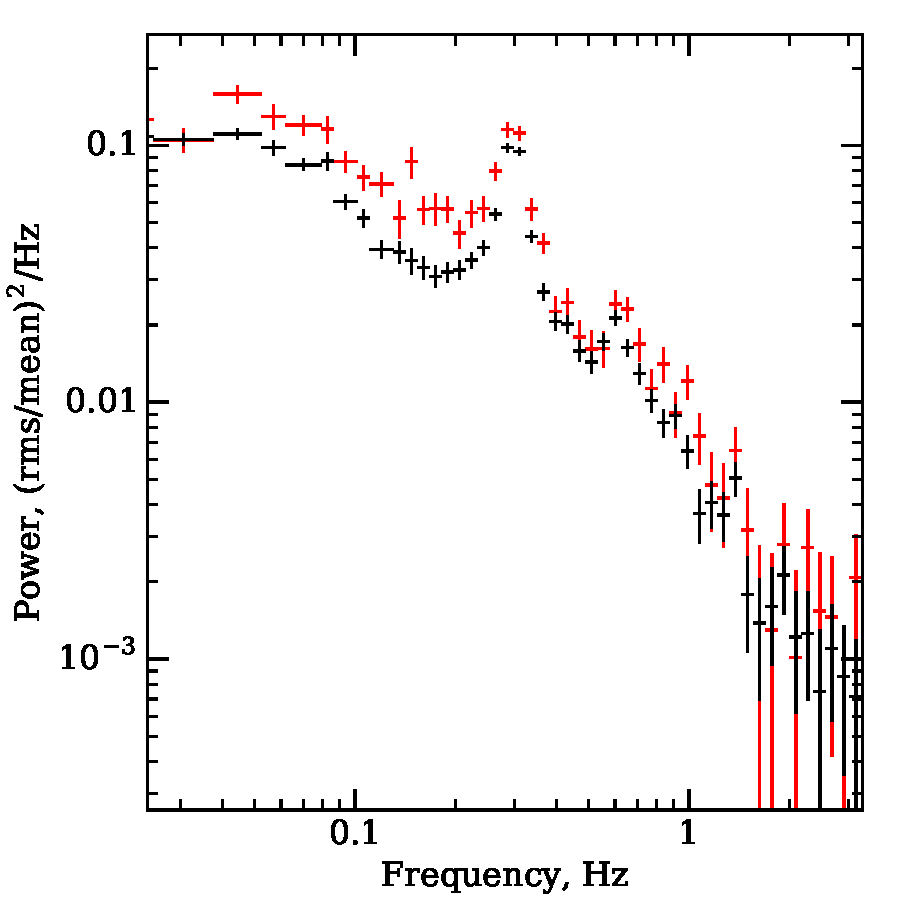
\includegraphics[width=\columnwidth]{folded_cospectr2.pdf}
        \caption{Cross-spectrum of the observations, obtained by scaling frequency to conserve QPO position.
        Black crosses obtained from the all data sets, while red crosses are from sets I, II, IV, and V, in which QPO subharmonics was most prominent.}
        \label{fig:cospec_tracked}
\end{figure}

The subharmonics seems to roam around the 1/2 QPO frequency, therefore we were not able to obtain it with a large significance on the tracked spectrum.

It should be noted that the changes in the QPO centroid position may contribute in the observed quality factor $Q$.
We can estimate the derivative of the QPO centroid position with time (by approximating $f_{\rm QPO}(time)$ with the straight line), which appears to be $\dot{f}_{\rm QPO} \approx 6.5\times10^{-6}$~Hz~s$^{-1}$. 
During an observation with the duration $\tau = 3000$~s even perfect QPO located at $f_{\rm QPO}=0.3$~Hz is observed with the quality factor $Q \approx \dot{f_{\rm QPO}}\tau/f_{\rm QPO} \approx 0.065$, which is of order of the Q estimations obtained from the observations with \ref{eq:complex_fit} model.
In order to better estimate the QPO quality factor, we separated each of the 13 observations on 82~s time-series. 
Power spectra in each observation we fitted simultaneously substituting in the model~\ref{eq:complex_fit} instead of the QPO centroid frequency $f_{\rm qpo} + (t - t_{\rm mid})\dot{f}_{\rm qpo}$, with $\dot{f}_{\rm qpo}$ being the free parameter, $f_{\rm qpo}$ QPO centroid position estimated for the model\ref{eq:complex_fit}  and $t_{\rm mid}$ middle of the data set observation time interval. 
Inside each data set we obtained the QPO centroid changing speed consistent with the estimation obtained from the general trend, nevertheless the median quality factor, obtained in this model appears to be $\sim7\times10^{-2}$ - i.e. compatible with the previous estimations (see Table~\ref{tab:timing}). 




\begin{figure*}
        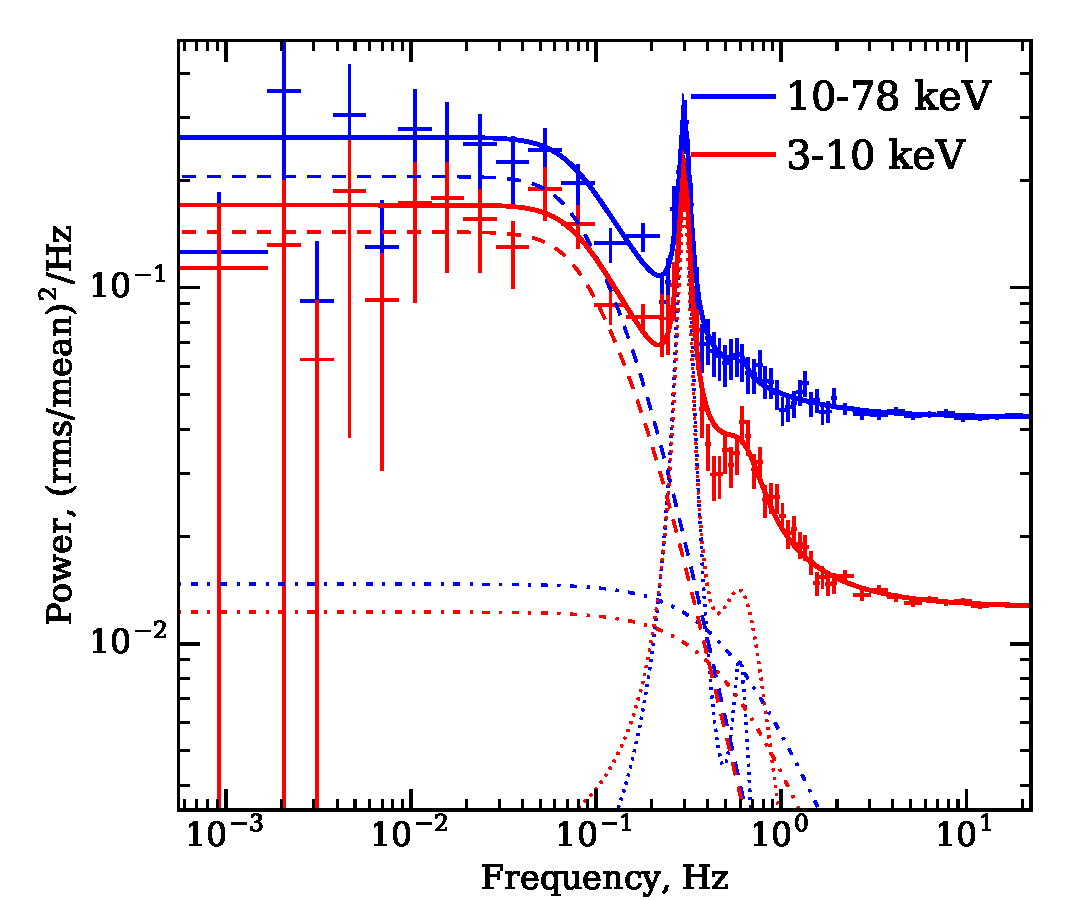
\includegraphics[trim=0 0 0 0.65cm, clip, width=\columnwidth]{NuFirst.pdf}
        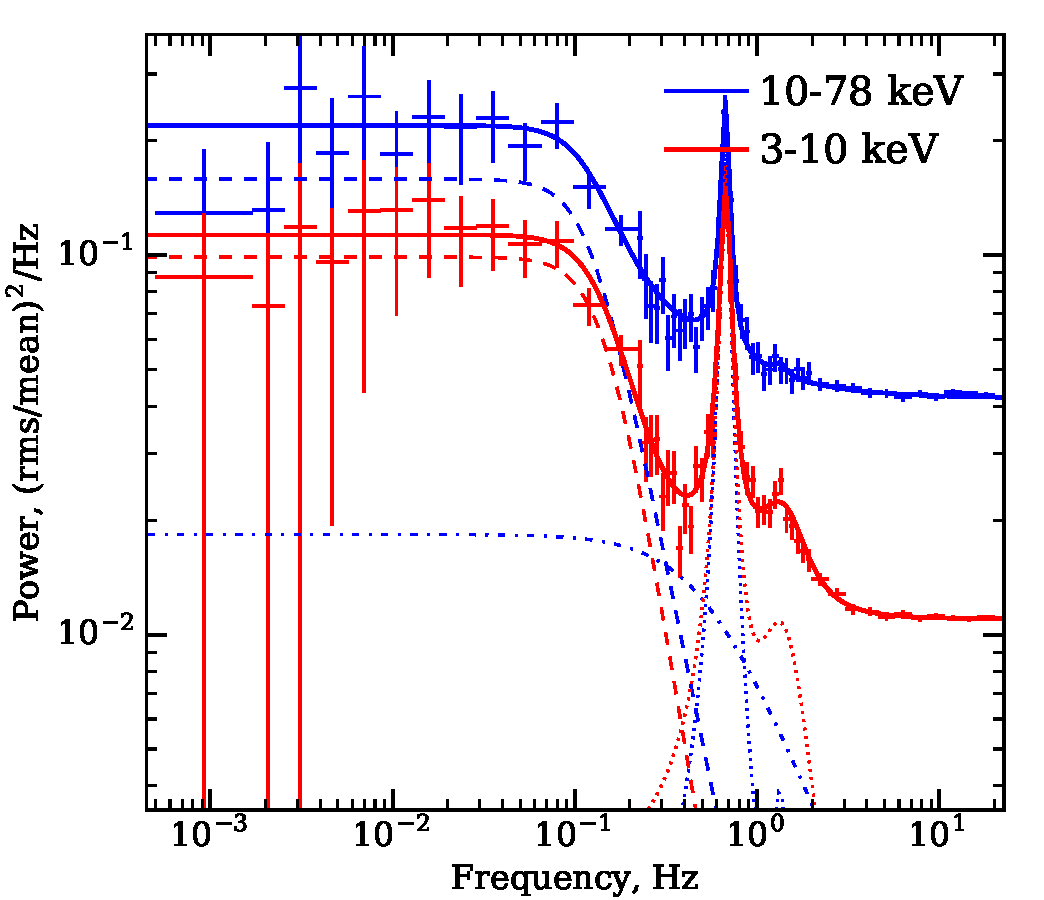
\includegraphics[width=\columnwidth, height = 0.83\columnwidth]{NuLast.pdf}
        \caption{On the left panel power spectra obtained in the soft (red) and hard (black) bands at the beginning of {\it NuSTAR} observation. 
        On the right column same spectra obtained at the end of the observation.}
        \label{fig:ps_example}
\end{figure*}

In Table \ref{tbl:ps_fit_parameters} one can fined obtained fit parameters for the 13 separate uninterrupted {\it NuSTAR} time series.

\subsection{Coherence}

    Power spectra of XBs are often have a complex shape with broad band noise and QPO like features, and numerous different models of these system were suggested to explain each particular feature. 
\citep{vaughan97} suggested to use coherence between different energy bands in order to obtain additional information on the source time properties. 
They define coherence as 
\begin{equation}
    C(f) = \frac{|<H(f)^*S(f)>|^2}{<|H(f)|^2><|S(f)|^2>}
    \label{eq:nowak_coh}
\end{equation}
where $H(f)$ and $S(f)$ are Fourier function of time series in hard and soft bands correspondingly. 
This function demonstrates the similarity of stochastic time signal in both bands. 
Different models of the XBs variability formation suggest that the signal in two energy bands can be partially independent, while the shape of the power spectra is conserved.
It appears that in many sources coherence between soft and hard X-ray bands is close to unity \citep{nowak99, wijnands01, eijden17}, in contrary to different models predictions \citep[see, discussion in][]{vaughan97}.

Following method \citep{nowak99} we estimated correlation of \grs\ light-curves obtained in the soft and hard energy bands. 
Since for the timing analysis we use {\it NuSTAR} data, we adopt following energy bands for the soft and hard light-curves correspondingly: 3--10~keV (soft) and 10--79~keV (hard).

In contrast to the \citep{nowak99} study, net count rate, obtained in \grs\ {\it NuSTAR} observation is {\bf 160~s$^{-1}$}, it follows that approximately quarter of the total variability power is due to the Poisson noise. 
As was discussed in \citep{nowak99} the correlation of two independent time series demonstrates large errors on the frequencies dominated with Poisson noise, due to the random walk in the 2-D complex space.
We also found, that the correlation of the light-curves obtained from {\it NuSTAR} is subjected by the dead-time and crosstalk effects between the energy bands.
In order to eliminate this effects, following the recipe suggested in \cite{2015ApJ...800..109B} for power spectra estimation, we find crossproducts of the light-curves Fourier functions obtained on the different modules - e.g. correlations of the light-curve obtained in the soft band on the FPMA module with the light-curve in the hard band obtained in the FPMB and vice versa.
Obtained correlation does not contain polluting signal from the blocking dead time. 

After that, as explained in \citep{nowak99}, one should find the amplitude of the fully coherent signal $<|H(f)|^2><|S(f)|^2>$ in order to estimate coherence of the signals. 
There is several different options, which one can be use to estimate this normalization:
\begin{enumerate}
        \item Use observed of the power spectra in each energy band. 
                 The drawback of this method is that power spectra contain Poisson noise component constant on all frequencies and dominating over the source variability on high frequencies. 
                 Thus, since Poisson noise is not coherent,  if one use this normalization as a denominator in Eq.~\ref{eq:nowak_coh} coherence estimation will be dumped on the value equal to the ratio of the Poisson noise to the source signal power on each frequency.
        \item Instead of the observed power spectra, one can use approximation of the power spectra with analytical models. 
                Poisson noise component can be discarded in analytical model, thus only source signal is conserved. 
                The drawback is that due to the Dead time effects Poisson noise has a complex form and can not be easily estimated with simple model.
        \item Use coherent part of the Fourier function of light curves in two modules \citep{2015ApJ...800..109B} or it's approximation with the analytical function. 
                It should be noted, that obtained coherent part of the ${\rm re}(H_{\rm A}(f)^*H_{\rm B}(f))$ has complex statistic which not restricting negative values, which must be ignored or modified thus affecting result.  
                We also found, that for short time series, one should use more complex likelihood criterion in order to fit coherent signal with analytical functions, since the statistic is still far from Gaussian and obtained fits are often unstable.
\end{enumerate}

\begin{figure}
    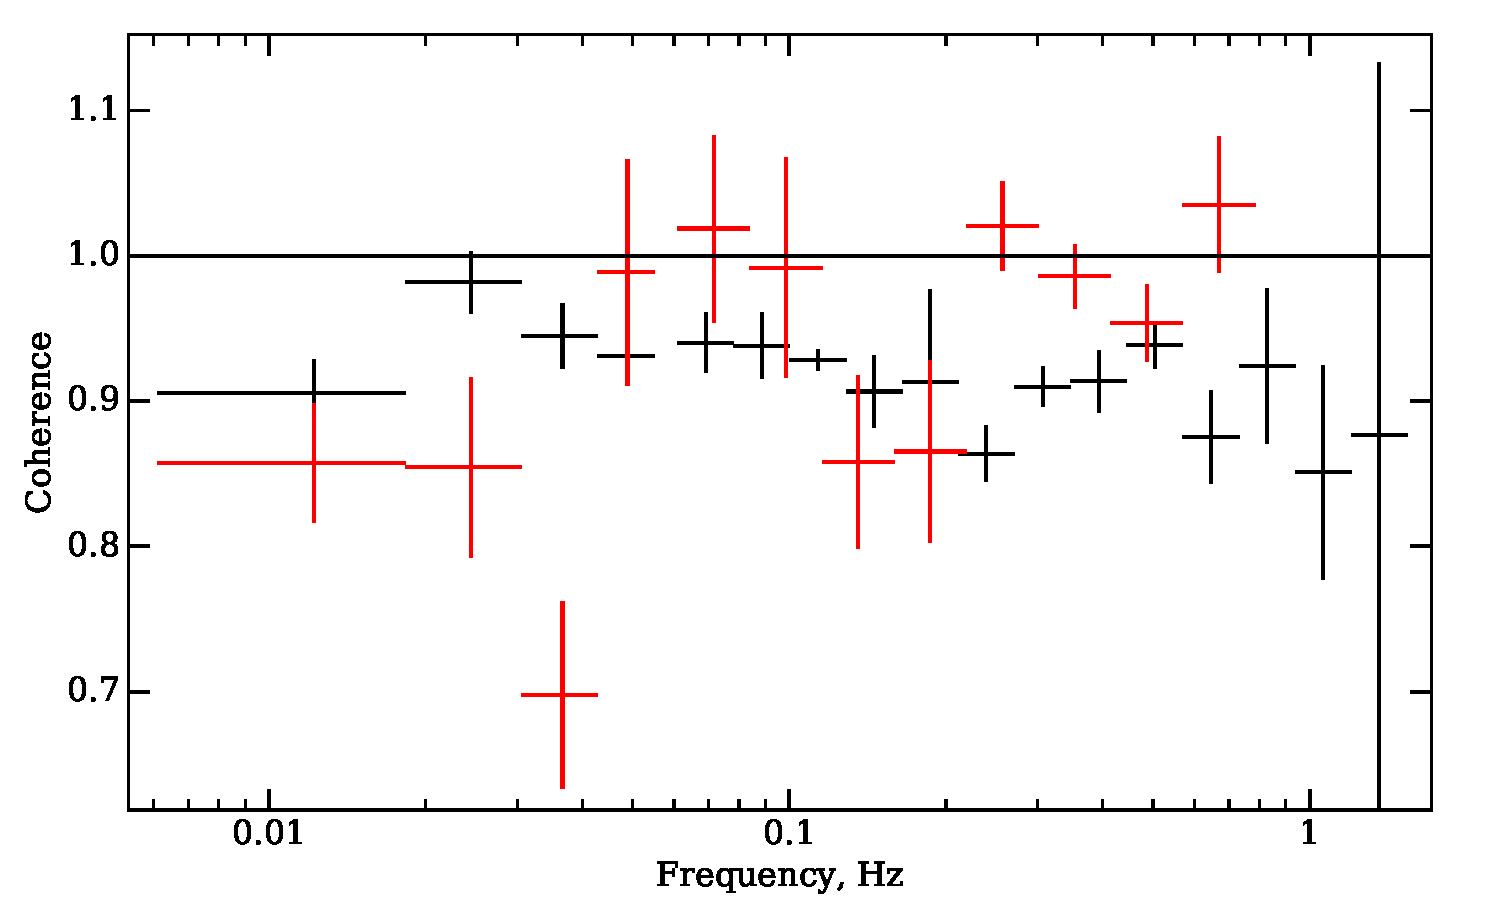
\includegraphics[width=\columnwidth]{coherence_3.pdf}
    \caption{Coherence between the soft (3--10~keV) and hard (10--78~keV) energy bands as a function of frequency. 
     Black crosses  represent estimations made with the both cross components and power spectra are obtained from data.
     Red crosses obtained from the cross component obtained from divided by the power spectra analytical models with Poisson noise components subtracted.}
    \label{fig:coherence}
\end{figure}


On Figure~\ref{fig:coherence} presented measured coherence between hard and soft bands on the frequencies up to $\sim1$~Hz. 
Two methods were used to obtain coherence, first we use cross spectra as an assessmnet to the signals variability power in each band (black crosses on Figure~\ref{fig:coherence}, and second we used analytical models obtained via fitting dirrect power spectra and subtracting Poisson noise component (red crosses). 
The data after that was rebinned it to the logarithmical bins and the error were estimated statisticaly as a standard deviation of values in each bins. 
Coherence in the first few frequency channels were not binned, instead, observations were split on several subsets, coherence in this subsets were obtained and standard deviation of that samples were estimated.
Since we have only 13 separate observations, standard deviation was obtained with very few degrees of freedom and therefore is underestimated. 

We found that, while coherence is of order of unity in the close energy bands (3--5 to 5--8~keV and 8--15 to 15--78~keV) it drops down to $\approx0.8$ between hard and soft bands (3--5 to 15--78~keV) which is not similar to results obtained for Cyg X-1 \citep{nowak99}.
It worth nothing, that the energy spectrum obtained with {\it NuSTAR} can be explained with two absorbed spectral components (powerlaw plus relativisticly broadened fluorescent Fe K$\alpha$ line), see Sec.~\ref{sec:spec}.
There is no clear changes in the coherence on the QPO frequency, i.e. soft and energy bands is not fully coherent. % despite they thought to be produced in the same place according to the geometrical model of the QPO origin \citep{ingram09,ingram11}.
%This behaviout seems tagling since {\it NuSTAR} energy spectrum can be described with only absorbed power law continuum and relativistically broadened Fe K$\alpha$ line.
%The power spectra, in hard and soft energy bands, have very similar shape (see Fig.~\ref{fig:ps}), therefore the processes, responsible for variability generation should be localized near the zones responsible for emission in each of these bands. 


%Since coherence is dumped on all frequencies one could suggest, that 0
%This method allows to rid out of the complex high frequency features connected with the cross-talk in the energy bands and blocking dead time effects.

%There is a drawback with this method, 
%Since Poisson noise in the two considered energy bands is independent, correlation of the light-curves computed with the eq.4 from \cite{Nowak99} is dumped, and tends to zero on the frequencies where Poisson noise dominates over the source variability.
%Therefore, to obtain proper estimates on the correlation function and phase lags between soft and hard flux, instead of the product of estimates of power spectra in two energy bands as denominator we are use analytical model $P_{h}(f)\cdotP_{s}(f)$ describing corresponding power spectra. 
%Here $P_h(f)$ and $P_s(f)$ - analytical function, approximating the power spectra in soft and hard bands.
%We found, that the power spectra in this bands are very similar to each other and can be fitted on the frequencies above 0.01~Hz with the following function:


%We found, that our estimate on the coherence, growths significantly on the frequencies above $\sim2$~Hz, where Poisson noise begins to dominate over the source intrinsic variability.
%This can be explained with the uncertainty of the obtained model parameters or its simplicity. 
%We found that for both soft and hard bands, obtained fits suggest very abrupt drop in power between the QPO and low-frequency plateau, it leads to very steep index of the power-law component. 
%Therefore growth of the coherence estimates on the higher frequencies is due to the underestimation of the source intrinsic variability on the corresponding frequencies.

%We found, that, similarly to different XBs, light curves in the hard and soft bands demonstrate strong correlation up to the high frequencies, however, we were not able to estimate properly coherence above 2~Hz due to the Poisson noise.

\subsection{Phase lags}
    
Following \citep{1997ApJ...474L..43V} we estimate phase lag as an angle of mean product of the light curves Fourier harmonics from one energy bands to the conjugated Fourier harmonics of second energy band. 
\begin{equation}
        P_{\rm hs} = F_h(f)^{*}F_s(f)
\end{equation}
We can imagine that each light curve from a sample consist of stochastic noise and coherent signal $F_{\rm h[s]} = ne^{-i\alpha}$, where $i$ - is complex unit, k - amplitude of the Fourier harmonic and $\alpha$ its phase.
Amplitudes of each harmonic in that case are distributed with the Normal distribution with zero mean, and divergence equal to the square power in particular frequency band. 
The probability density function (PDF) of the product of two Normal distribution described with the modified Bessel function of second kind with 0-th order. 
Result of the product of two Foruier harmonics can be represented ad a sum of four complex numbers, amplitude of each is distributed with PDF having a form of modified Bessel function, phases of three of these numbers distributed uniformly, and phase of the last one is distributed nonuniformly with mean equal to real phase shift between two coherent signals.
We can now determine the ``phase axis'' as the axis along the mean complex value of the Sample.
Distribution of the points relative to the ``phase axis'' obviously should be symmetrical, and along it should be assymetric and shifted towards the mean complex value of the sample.
If we now rotate all the obtained complex Fourier harmonics in our sample along this axis $\frac{<P_{\rm hs}^{*}>P_{\rm hs}}{|<P_{\rm hs}>|}$, real part of each value is the projection on the ''phase axis'' and imaginary part is projection on the perpendicular axis. 
We found that the distribution of the projected on the ''phase axis'' values is closely resembles assymetric Laplace distribution and the distribution of the points projected on the perpendicular axis resembles symmetric Laplace distribution. 
Bearing this in mind we estimate mean value for each of the four distributions (positive real, negative real, positive imaginary and negative imaginary) and assess variances of this distribution.
Since we accepted that each of these distribution has a PDF close to exponential we take their variance as a variance of $\chi_2^{\rm 2N}$ distribution, where $N$ - is a number of entities in the each sample. 
After that we accept the error on the phase to be equal $\pi$ if the mean of positive real sample is less than the square root of the sum of the positive and negative real samples variances, otherwise we take it to be equal
\begin{equation}
        \Delta \phi = atan{\left(\frac{\sqrt{v_{i-}^2 + v_{i+}^{2}}}{m_{r+} - m_{r-} - \sqrt{v_{r+}^2 + v_{r-}^2}}\right)}
\end{equation}



    Error assessment for the phase lag points position 


    Most of the models of the accretion flow which describe variability and energy spectra formation, suggest the time lag between the signals in different energy bands. 
For example in some models of the energy spectra formation, time lag is naturally arise due to the geometry of the corona and properties of the inverse Comptonization process \citep[see, e.g.][]{kotov01}.
Phase lag is also suggested from the propagating fluctuations model - hard photons are emitted from the inner parts of the accretion flow from the perturbations, which initially were born in the outer parts of the disk were produce soft emission.  

It also was found, that phase lag of XBs, probably depends on the system inclination angle \citep{eijeden17}, it also definitely contain information about the characteristic times of the system, and therefore can be proxy to the compact object mass \citep{}. 

Phase lags can be estimated as a product of the mean phase of the set of Fourier spectra and the corresponding frequency:
\begin{equation}
                \tau = \frac{\phi(f)}{2\pi f}\\
\end{equation}
\begin{equation}
        \phi(f) = <arccos{\left(\frac{re(<F_{\rm h}^{*}(f)F_{\rm s}(f)>)}{|F_{\rm h}^{*}(f) F_{\rm s}(f)|}\right)}>
        \label{eq:phase_lag}
\end{equation}
here, $F_h(f)$ and $F_s(f)$ are Fourier functions of the light-curves in the hard and soft bands, $\phi(f)$ is the phase lag. 

%Due to the significant fraction of the Poisson noise in each observation we were not able to obtain phase lag for them.
We found that phase lag on each frequency is generally conserved along the observation.
In order to improve significance we compute phase lag for all 13 time series.
Obtained phase lag for frequencies from $10^{-2}$~Hz to 100~Hz is presented in Figure~\ref{fig:phase_lag}.
As follows from the Eq.~\ref{eq:phase_lag} we compute phase shift between the phases of the Fourier harmonics in hard and soft lightcurves, therefore negative phase lag corresponds to the hard lag.
It Follows from Figure~\ref{fig:phase_lag} that there is soft lag on low frequencies which transforms in to the hard lag on frequencies grater than QPO frequency. 

\begin{figure}
        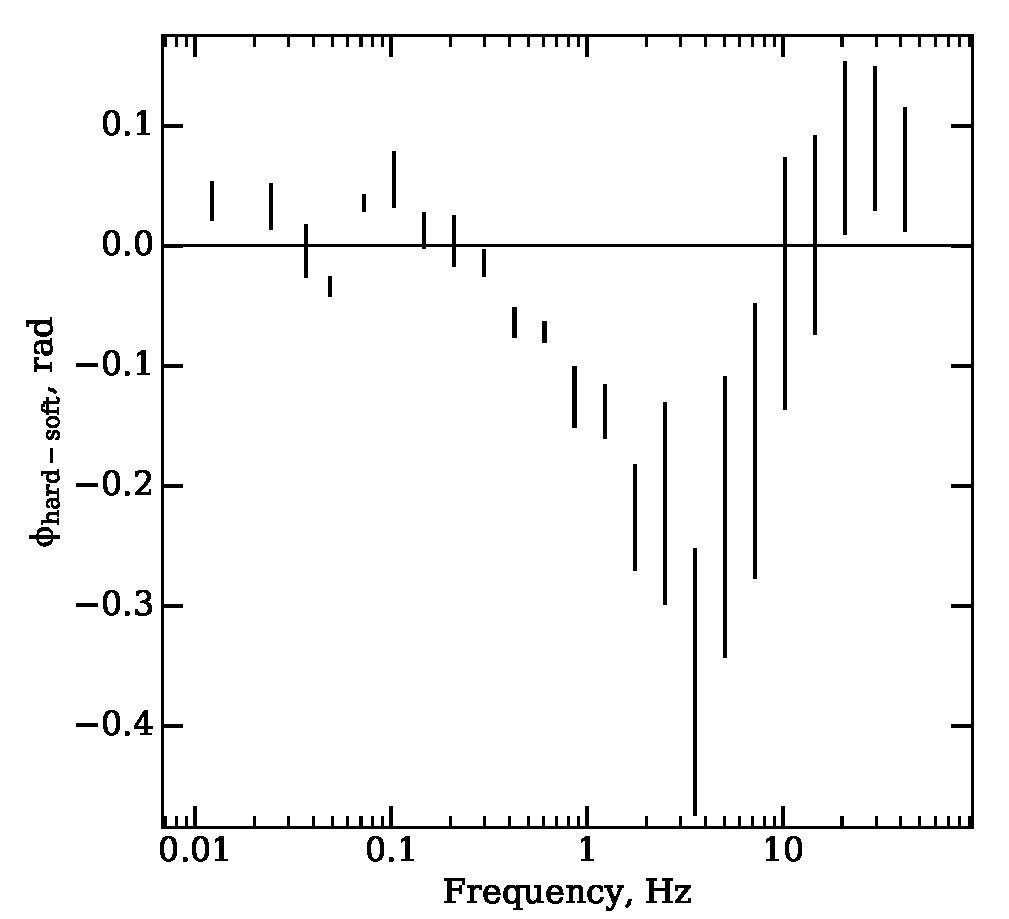
\includegraphics[width=\columnwidth]{Phase_lag.pdf}
        \caption{Phase lag between the hard (10--78~keV) and soft (3--10) energy bands in \grs}
        \label{fig:phase_lag}
\end{figure}

\subsection{timinig discussion}
We found that the total power in the second QPO harmonic in the soft band is comparable to the total power in the main harmonic, in the hard band second harmonic is $\approx3$ times less powerfull than the main. 
Total power of the harmonics growing with the source count-rate and QPO frequency in the soft and hard energy bands (see Table~\ref{tab:timing}). 
%If the QPO has geometrical origin - i.e. it's due to the change of the view on the some statical illumination pattern like in the \citep{IVK09} model, than this pattern is more complex in the soft energy band. 

%If the QPO is due to the changing of our field of view on some static pattern, like in the \citep{ivk09} model, than it follows that QPOs in this bands have different origin - i.e. QPO in the soft band is due to the scattering of the photones from precessing corona, while QPOs  reflection of the ro

\section*{Acknowledgments}

%--------------------------------------------------------------------------------
\bibliographystyle{astron}
\bibliography{author_en.bib,coherence.bib}
\bsp	
\label{lastpage}
\end{document}
